\begin{frame}{Sistemas de bases de datos (SBD)}
  
    \centering
    \begin{tikzpicture}<1->
        \node at (0,3.7) {\tiny \bf {Usuario}} ;
        \node[inner sep=0pt] (user) at (0,3) {
            
\includegraphics[width=1.3cm]{img/user.png}
        };

        \node at (3,3.7) {\tiny \bf {Aplicaci\'on}} ;
        \node[inner sep=0pt] (desktop) at (3,3) {
            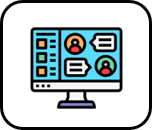
\includegraphics[width=1.3cm]{img/desktop.png}
        };

        \node at (6,3.7) {\tiny \bf {SGBD}} ;
        \node[inner sep=0pt] (dbms) at (6,3) {
            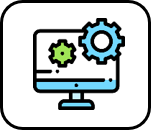
\includegraphics[width=1.3cm]{img/dbms.png}
        };

        \node at (9,3.7) {\tiny \bf {Base de datos}} ;
        \node[inner sep=0pt] (database) at (9,3) {
            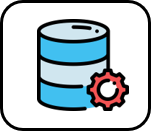
\includegraphics[width=1.3cm]{img/database.png}
        };

        \draw[<->,thick] (user.east) -- (desktop.west);
        \draw[<->,thick] (desktop.east) -- (dbms.west);
        \draw[<->,thick] (dbms.east) -- (database.west);
    \end{tikzpicture}
    \vspace{10pt}
    \begin{block}<2->{}
        \begin{quote}
            ``Un \textcolor{red}{sistema de base de datos} es un 
            \textcolor{red}{sistema computacional de mantenimiento de registros}, 
            que se dise\~na para manejar grandes cantidades de informaci\'on."
            \hspace{1em plus 1fill}---C. J. Date
        \end{quote}
       
    \end{block}

    \begin{block}<3->{Funciones}
        \begin{columns}[T]
            \begin{column}{0.48\linewidth}
                \begin{itemize}
                    \item Insertar datos
                    \item Editar datos
                \end{itemize}
            \end{column}
            \begin{column}{0.48\linewidth}
                \begin{itemize}
                    \item Eliminar datos
                    \item Consultar datos
                \end{itemize}
            \end{column}
            
        \end{columns}
    \end{block}
  
\end{frame}